%------------------------------------------------------------------------------
% Author(s):
% Varaun Ramgoolie
% Copyright:
%  Copyright (C) 2020 Brad Bachu, Arjun Mohammed, Nicholas Sammy, Kerry Singh
%
%  This file is part of Applied-Mathematics-Unit2 and is distributed under the
%  terms of the MIT License. See the LICENSE file for details.
%
%  Description:
%     Year: 2008 June
%     Module: 1
%     Question: 1 
%------------------------------------------------------------------------------
\usetikzlibrary{patterns}

\begin{subquestions}
	
%------------------------------------------------------------------------------
% 1 a -------------------------------------------------------------------------
%------------------------------------------------------------------------------

\subquestion

The objective function that we want to maximize is,

\begin{equation}
	P=15x + 27y \,. 
\end{equation}

Using $x$ as the number of units of product X and $y$ as the number of units of product Y, our inequalities are,

\begin{align}
	x & \geq 0 \,, \nn \\
	y & \geq 0 \,, \nn \\
	6x + 9y & \leq 360 \,, \nn \\
	15x + 9y & \leq 675 \,.
\end{align}

%------------------------------------------------------------------------------
% 1 b -------------------------------------------------------------------------
%------------------------------------------------------------------------------

\subquestion

The feasible region is shaded in the graph below.

\begin{center}

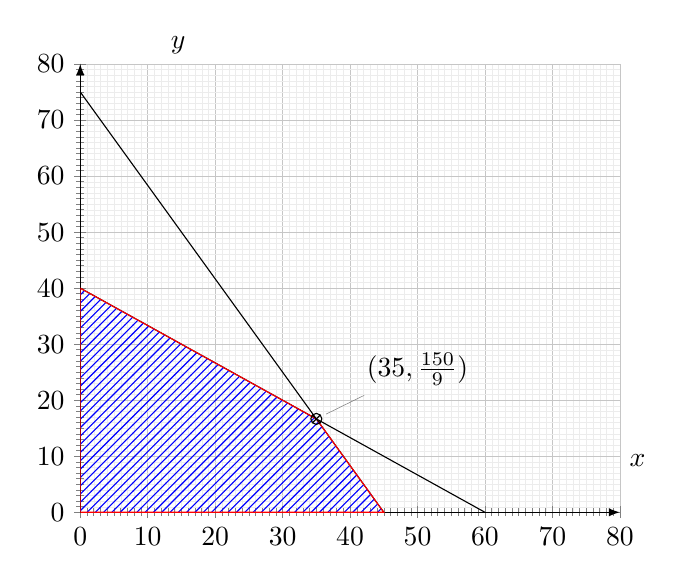
\begin{tikzpicture}
	\begin{axis}
		[
		xmin=-0,xmax=80,
		ymin=0,ymax=80,
		grid=both,
		grid style={line width=.1pt, draw=darkgray!10},
		major grid style={line width=.2pt,draw=darkgray!30},
		axis lines=left,
		minor tick num=9,
		enlargelimits={abs=0},
		axis line style={-latex},
		samples=100,
		domain = -20:20,
		ytick={0,10,...,80},
		xtick={0,10,...,80},
		xlabel={$x$},
		ylabel={$y$},
		x label style={at={(axis description cs:1,0.15)},anchor=north west},
		y label style={at={(axis description cs:0.15,1)},anchor=south west, rotate=-90}
		]
		
		\addplot [mark=dot] coordinates{(60, 0)  (0,40)};
		
		\addplot [mark=dot] coordinates {(45,0) (0, 75)};
		
		\addplot [red,pattern=north east lines,pattern color=blue] coordinates {(0,40) (35, 150/9) (45, 0)} \closedcycle;	
		
		\node [pin=30:{$(35, \frac{150}{9})$}] at (axis cs:(35, 150/9) {};
		
		\addplot [mark=otimes] coordinates{(35, 150/9)};
				
	\end{axis}	
\end{tikzpicture}

\end{center}

%------------------------------------------------------------------------------
% 1 c -------------------------------------------------------------------------
%------------------------------------------------------------------------------

\subquestion

From \rdef{mod1:defn:TourOfVertices}, we can calculate $P$ by,

\begin{align}
	\text{Using (0,40)} \,, \nn \\
	P & = 15x + 27y \,, \nn \\
	  & = (15 \times 0) + (27 \times 40) \,, \nn \\
	  & = 1080 \,. \label{2008:q1:eqn:Profit} \\
	\text{Using (35, $\frac{150}{9})$} \,, \nn \\
	P & = 15x + 27y \,, \nn \\
	  & = (15 \times 35) + (27 \times \frac{150}{9}) \,, \nn \\
	  & = 705 \,.    \\		  
	\text{Using (45,0)} \,, \nn \\
	P & = 15x + 27y \,, \nn \\
	  & = (15 \times 45) + (27 \times 0) \,, \nn \\
	  & = 675 \,. 
\end{align}

Thus, from \req{2008:q1:eqn:Profit}, the maximum value of $P$ is $1080$.

\end{subquestions}

